\section[Perceptron Algorithm]{Perceptron Algorithm}

\subsection[History]{History}

\begin{frame}{History}
	\begin{itemize}
		\item \textbf{1943}: McCulloch (neurophysiologist) and Pitts (mathematician) establish the first mathematical model of a \textbf{human neuron}. It is a binary and purely logical model. The parameters are fixed manually. They seek to show that the human brain is a computing machine and demonstrate how to program logic gates (AND, OR, NOT) using this model.
		\pause
		\item \textbf{1948}: Hebb (neuropsychologist) was the first to hypothesize that the brain was plastic. At the time, it was believed that connections between neurons were established once and for all at birth. He thus theorizes that connections between neurons strengthen during learning: \textit{"Neurons that fire together, wire together."}
		\item \textbf{1958}: Rosenblatt (psychologist) draws inspiration from Hebb's work to improve McCulloch and Pitts' vision. He comes up with the idea to update the mathematical neuron's parameters based on the error made by that same neuron. He invents the first learning algorithm: the Perceptron.
	\end{itemize}
\end{frame}

\begin{frame}{History}
	\begin{itemize}
		\item \textbf{1969}: Minsky and Papert formally demonstrate that the Perceptron algorithm cannot program an exclusive OR (XOR) gate. They also show that multiple neurons would actually be required to program such a gate, but that the learning algorithm no longer worked in that case. This brings research on the Perceptron to a halt.
		\pause 
		\item \textbf{1986}: Rumelhart, Hinton, and Williams publish an article presenting the gradient backpropagation algorithm, which allows training a Multilayer Perceptron. They successfully train a neural network that replicates an exclusive OR logic gate. Other scientists made prior contributions to this article: Linnainmaa (1970), Werbos (1974), and LeCun (1985).
	\end{itemize}
\end{frame}

\subsection[Perceptron Intuition]{Perceptron Intuition}

\begin{frame}{Geometric Approach}
	In a plane defined by the variables $X_1$ and $X_2$, the equation of a line $\mathcal{D}$ is given by:
	
	\begin{equation*}
		w_1 \cdot x_1 + w_2 \cdot x_2 + w_3 = 0
	\end{equation*}
	
	\vspace{0.3cm}
	
	With $w_1$, $w_2$, and $w_3$ being the coefficients of the line.
	
	\begin{figure}
		\centering
		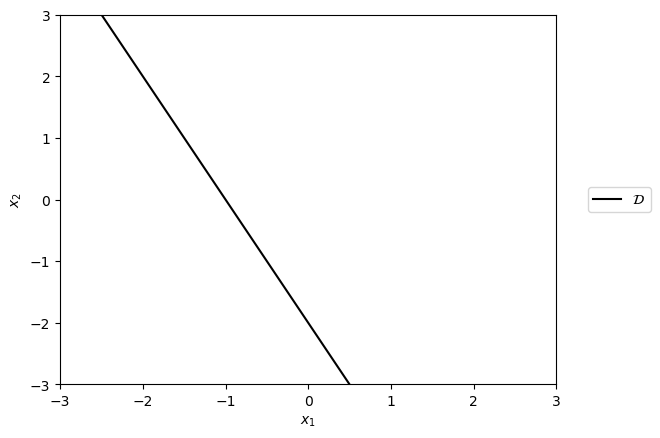
\includegraphics[height=0.3\linewidth]{Images/droite01}
		\label{fig:droite01}
	\end{figure}			
	
\end{frame}

\begin{frame}{Space Regions}
	We denote the following quantity as $z$:
	
	\begin{equation*}
		z = w_1 \cdot x_1 + w_2 \cdot x_2 + w_3
	\end{equation*}
	
	The line $\mathcal{D}$ \textbf{separates} the space into two distinct regions:
	
	\begin{itemize}
		\item A region where $z > 0$.
		\item A region where $z < 0$.
	\end{itemize}
	
	\vspace{0.2cm}
	
	On the line $\mathcal{D}$, $z$ is zero by definition.
	
	\begin{figure}
		\centering
		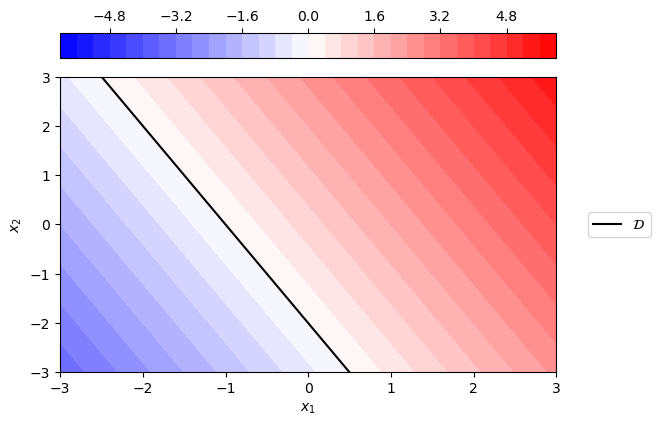
\includegraphics[height=0.3\linewidth]{Images/droite02}
		\label{fig:droite02}
	\end{figure}
	
\end{frame}

\begin{frame}{Position of a Point}
	We denote a point $P$ with coordinates $\left( x_1^{(P)}, x_2^{(P)} \right)$:
	
	\begin{equation*}
		z^{(P)} = w_1 \cdot x_1^{(P)} + w_2 \cdot x_2^{(P)} + w_3
	\end{equation*}
	
	\begin{figure}
		\centering
		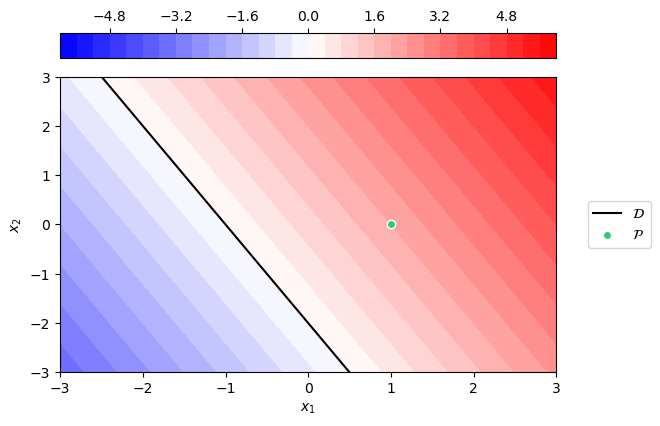
\includegraphics[height=0.4\linewidth]{Images/droite03}
		\label{fig:droite03}
	\end{figure}
\end{frame}

\begin{frame}{Classification Problem}
	In a \textbf{linearly separable} binary classification problem:
	
	\begin{itemize}
		\item We have multiple points: $\mathcal{P} = \left\{ \left( x_1^{(i)}, x_2^{(i)}\right) \right\}_{i=1}^n$.
		\item Each point (or observation) is associated with a class $y^{(i)} \in \{0, 1\}$.
		\item We look for a line $\mathcal{D}$ that \textbf{perfectly separates} the observations of the two classes.
	\end{itemize}
	
	\vspace{0.3cm}
	\pause
	
	This is equivalent to finding a line $\mathcal{D}$ such that \textit{all} observations of class $K = 1$ have a \textbf{positive} quantity $z$ and \textit{all} observations of class $K = 0$ have a \textbf{negative} quantity $z$.
	
	\vspace{0.3cm}
	\pause
	
	To simplify the notation of the Perceptron algorithm, we will consider \textbf{augmented data} for $x$:
	
	\begin{equation*}
		x^{(i)} = \left( x_1^{(i)}, x_2^{(i)}, 1\right)
	\end{equation*}
\end{frame}

\begin{frame}{Rosenblatt's Perceptron Algorithm}
	For a linearly separable binary classification problem:
	\begin{enumerate}
		\item We randomly initialize the coefficients $w_1$, $w_2$, $w_3$.
		\pause
		\item Main loop: \textbf{epochs}
		\pause
		\begin{itemize}
			\item For each observation $i$:
			\begin{itemize}
				\item We compute the quantity $z^{(i)} = w_1 \cdot x_1^{(i)} + w_2 \cdot x_2^{(i)} + w_3 \cdot 1$.
				\pause
				\item We compute the sign of this quantity, denoted as $\sign{z^{(i)}}$:
				\begin{equation*}
					\sign{z^{(i)}} = 
					\begin{cases}
						1 & \text{if} \; z^{(i)} \ge 0 \\
						0 & \text{otherwise}
					\end{cases}
				\end{equation*}
				\item We compare $\sign{z^{(i)}}$ to the true class $y^{(i)}$ and adjust with a small learning rate $\alpha \in \mathbb{R}$, for all $j = 1, 2, 3$:
				\begin{equation*}
					w_j \leftarrow w_j + \alpha \cdot \left[y^{(i)} - \sign{z^{(i)}}\right] \cdot x_j^{(i)}
				\end{equation*}
			\end{itemize}
			\pause
			\item We repeat until all observations have been processed.
		\end{itemize}
		\pause
		\item We repeat step 2 until all observations are correctly classified: $\operatorname{sign}(z^{(i)}) = y^{(i)} \; \forall \; i=1, 2, \cdots, n$.
	\end{enumerate}
\end{frame}

\begin{frame}{Geometric Interpretation of the Perceptron Algorithm}
	Suppose we have an observation $i$ such that $y^{(i)} = 0$ and $z^{(i)} > 0$. Since the sign of $z$ does not match the true class, the Perceptron algorithm performs an update from state $k$ of the line's coefficients:
	
	\begin{equation*}
		\begin{aligned}
			w_j^{(k+1)} 
			&= w_j^{(k)} + \alpha \cdot \left[ y^{(i)} - \sign{z^{(i)}}\right] \cdot x_j^{(i)} \\
			&= w_j^{(k)} - \alpha \cdot x_j^{(i)}
		\end{aligned}
	\end{equation*}
	
	\begin{figure}
		\centering
		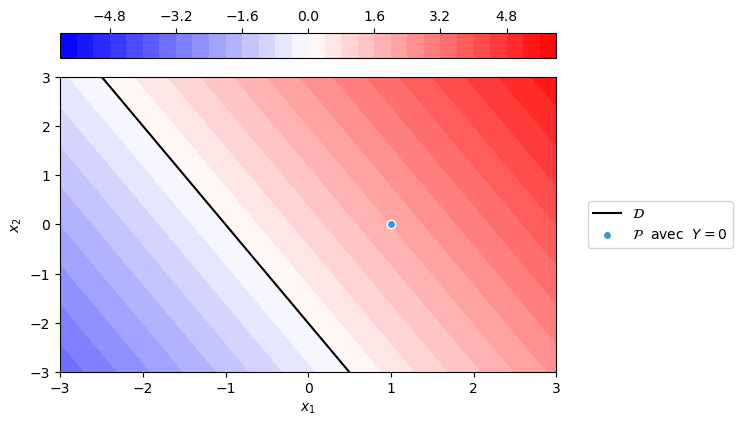
\includegraphics[height=0.3\linewidth]{Images/droite04}
		\label{fig:droite04}
	\end{figure}	
	
\end{frame}

\begin{frame}{Geometric Interpretation of the Perceptron Algorithm}
	By arranging the coefficients $w_j$ of the line into a column vector $w \in \mathcal{M}_{3,1}(\R)$ such that $w = \begin{pmatrix} w_1 & w_2 & w_3 \end{pmatrix}^T$, we then have:
	
	\begin{equation*}
		\left(z^{(i)}\right)^{(k)} = x^{(i)}  w^{(k)}
	\end{equation*}
	
	And:
	
	\begin{equation*}
		\begin{aligned}
			\left(z^{(i)}\right)^{(k+1)} 
			&= x^{(i)} w^{(k+1)} \\
			&= x^{(i)} \left[w^{(k)} - \alpha \left(x^{(i)}\right)^T\right] \\
			&= x^{(i)} w^{(k)} - \alpha x^{(i)} \left(x^{(i)}\right)^T \\
			&= \left(z^{(i)}\right)^{(k)} - \alpha \| x^{(i)} \|_2^2
		\end{aligned}
	\end{equation*}
	
\end{frame}

\begin{frame}{Geometric Interpretation of the Perceptron Algorithm}
	However:
	
	\begin{equation*}
		\alpha \| x^{(i)} \|_2^2 > 0
	\end{equation*}	
	
	Therefore:
	
	\begin{equation*}
		\left(z^{(i)}\right)^{(k+1)} < \left(z^{(i)}\right)^{(k)}
	\end{equation*}
	
	\begin{itemize}
		\item The line moves in such a way that the quantity $z$ decreases. The line $\mathcal{D}$ approaches the point representing the observation, then passes it so that it ends up in a zone where $z^{(i)} < 0$.
		\item When there are multiple observations, the line must move \textit{relatively} slowly so as not to overly degrade the positioning of the other points relative to the line: $\alpha$ must be small enough for the algorithm's stability.
	\end{itemize}
\end{frame}

\begin{frame}{Application to AND and OR Logic Gates}
	\begin{columns}
		\begin{column}{0.5\textwidth}
			\begin{figure}
				\centering
				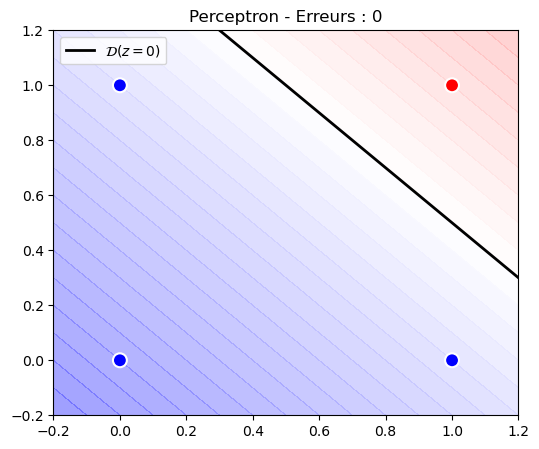
\includegraphics[height=0.8\linewidth]{Images/droite05}
				\label{fig:droite05}
				\caption*{AND Gate}
			\end{figure}			
		\end{column}
		\begin{column}{0.5\textwidth}
			\begin{figure}
				\centering
				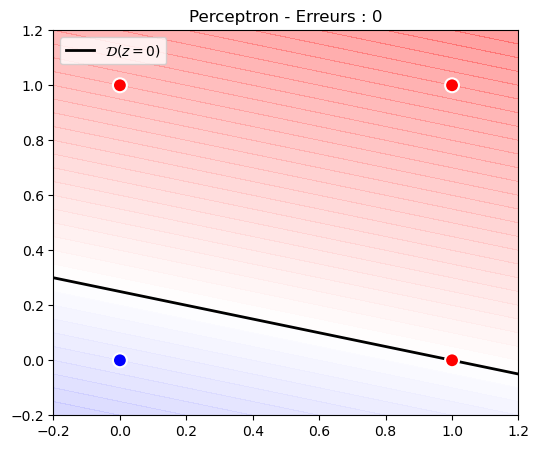
\includegraphics[height=0.8\linewidth]{Images/droite06}
				\label{fig:droite06}
				\caption*{OR Gate}
			\end{figure}			
		\end{column}
	\end{columns}	
\end{frame}

\subsection[Mathematical Neuron]{Mathematical Neuron}

\begin{frame}{Class Predicted by the Perceptron}
	For a given observation $i$, considering the augmentation $x^{(i)} = (x_1^{(i)}, x_2^{(i)}, \cdots, x_p^{(i)}, 1)$ organized in a row vector $x^{(i)} \in \mathcal{M}_{1,p+1}(\R)$ when the input space is $p$-dimensional: $\mathcal{X} \subset \R^p$, we can write the predicted class $\hat{y}^{(i)}$ from the input features and the coefficients of the line arranged in a column vector $w = (w_1, w_2, \cdots, w_p, w_{p+1})^T$ as follows:
	
	\begin{equation*}
		\hat{y}^{(i)} = \sign{x^{(i)} w}
	\end{equation*}
	
	\pause
	We can represent the sign of the quantity $z$ using the Heaviside step function $\sigma_h: \R \to \{0, 1\}$; the formulation then becomes:
	
	\begin{equation*}
		\hat{y}^{(i)} = \heaviside{x^{(i)} w}
	\end{equation*}
	
\end{frame}

\begin{frame}{Similarity to Logistic Regression}
	Rosenblatt's Perceptron predicts the class $\hat{y}^{(i)}$ with:
	
	\begin{equation*}
		\hat{y}^{(i)} = \heaviside{x^{(i)} w}
	\end{equation*}
	
	Logistic regression uses the logistic function $\sigma: \R \to (0, 1)$ instead of the Heaviside function:
	
	\begin{equation*}
		\hat{y}^{(i)} = \logistic{x^{(i)} w}
	\end{equation*}
\end{frame}


\begin{frame}{Reformulation of the Perceptron Algorithm}
	Without considering an augmentation of $x$, we can simply write $x^{(i)} = (x_1^{(i)}, x_2^{(i)}, \cdots, x_p^{(i)})$. An equivalent formulation of the Perceptron is then:
	
	\begin{equation*}
		\hat{y}^{(i)} = \heaviside{x^{(i)} w + w_{p+1}}
	\end{equation*}
	
	Which is more commonly written as:
	
	\begin{equation*}
		\hat{y}^{(i)} = \heaviside{x^{(i)} w + b}
	\end{equation*}
	
	Where $w$ is called the \textbf{weight} of the Perceptron and $b$ is called the \textbf{bias} of the Perceptron.
\end{frame}

\begin{frame}{Anatomy of Rosenblatt's Artificial Neuron}
	\begin{center}
		\begin{tikzpicture}[x=1.2cm, y=1cm, >=Stealth]
			
			% --- 1. Inputs ---
			\node[input] (x1) at (0, 2) {$x_1^{(i)}$};
			\node[input] (x2) at (0, 1) {$x_2^{(i)}$};
			\node (xdots) at (0, 0.2) {$\vdots$};
			\node[input] (xn) at (0, -0.7) {$x_p^{(i)}$};
			
			\node[anchor=south, font=\tiny\bfseries] at (x1.north) {Signals};
			
			% --- 2. The Soma (Summation + Activation) ---
			% Summation Block
			\node[neuron] (sum) at (3, 0.6) {$\displaystyle \sum$};
			
			% Activation Block (Heaviside)
			\node[neuron] (act) at (5, 0.6) {};
			
			% Drawing the Heaviside step inside the circle
			\draw[thick, blue] (4.75, 0.45) -- (5, 0.45) -- (5, 0.75) -- (5.25, 0.75);
			\node[anchor=north, font=\tiny, text=blue] at (act.south) {Heaviside};
			
			% --- 3. The Bias ---
			\node[input, fill=green!10, draw=green!60!black] (b) at (3, 2.3) {$b$};
			\draw[->, green!60!black, thick] (b) -- (sum) node[midway, right, bias] {+1};
			\node[anchor=west, font=\tiny, green!60!black] at (b.east) {Bias};
			
			% --- 4. Connections with Weights ---
			\draw[->] (x1) -- (sum) node[pos=0.4, above, weight] {$w_1$};
			\draw[->] (x2) -- (sum) node[pos=0.4, above, weight] {$w_2$};
			\draw[->, dashed, gray] (xdots) -- (sum);
			\draw[->] (xn) -- (sum) node[pos=0.4, below, weight] {$w_p$};
			
			% --- 5. Internal Transfer ---
			\draw[->, thick] (sum) -- (act) node[midway, above, font=\tiny] {$z^{(i)}$};
			
			% --- 6. Output ---
			\node (y) at (7, 0.6) {$\hat{y}^{(i)}$};
			\draw[->, thick] (act) -- (y);
			
			% --- Mathematical Annotations ---
			\node[anchor=north, font=\scriptsize, text=gray] at (sum.south) {
				$z^{(i)} = \sum_{j=1}^p w_j x_j^{(i)} + b$
			} ;
			
			% --- Zone Labels ---
			\draw[dashed, gray!40] (2, -1.5) -- (2, 3);
			\node[font=\tiny, gray] at (1, -1.3) {Synapses};
			\node[font=\tiny, gray] at (4, -1.3) {Soma (Cell body)};
			
		\end{tikzpicture}
	\end{center}
	
	Rosenblatt's perceptron (1958) consists of:
	
	\begin{itemize}
		\item A \textbf{linearity:} A simple weighted sum of the inputs to which a bias (activation threshold) is added.
		\item A \textbf{threshold function:} the Heaviside step function which represents the "All-or-Nothing" nature of a human neuron's activation. 
	\end{itemize}
\end{frame}

\begin{frame}{Limitations of the Perceptron}
	\begin{itemize}
		\item As discussed in the introduction, the Perceptron is unable to solve classification problems that are not \textbf{linearly separable}. This is the reason why it fell into oblivion for nearly 30 years (before the discovery of the gradient backpropagation algorithm).
		\item At the time of the Perceptron, \textbf{logistic regression} (which mathematically possesses a very similar formulation) was already known. However, these tools were used in different fields. Logistic regression was used in the medical field for statistical analyses, whereas the Perceptron was primarily an algorithm meant to demonstrate the computational nature of the human brain.
	\end{itemize}
\end{frame}